\chapter{Deseño do sistema}
\minitoc
\label{chap:diseno}
\vspace{0.5cm}

%%%%%%%%%%%%%%%%%%%%%%%%%%%%%%%%%%%%%%%%%%%%%%%%%%%%%%%%%%%%%%%%%%%%%%%%%%%%%%%%
% Objetivo: Exponer el diseño del PFC.                              %
%%%%%%%%%%%%%%%%%%%%%%%%%%%%%%%%%%%%%%%%%%%%%%%%%%%%%%%%%%%%%%%%%%%%%%%%%%%%%%%%

\lettrine{N}{este} capítulo exporase o deseño do proxecto baseándose no esquema
proporcionado pola planificación inicial: desde o deseño software e hardware do
sistema ata o estudo das posibles plataformas hardware, pasando por un terceiro
prototipo.

\section{Determinación}

 \subsection{Obxectivos}

 Establecéronse os obxectivos da fase de deseño do proxecto.

 \begin{itemize}
  \item Obter o deseño dunha gaita MIDI sen fíos en tempo real empregando
        software/hardware libre.
 \end{itemize}

 \subsection{Alternativas}

 Establecéronse posibles alternativas a eses obxectivos, aplicables no caso de
 que estes non se puidesen cumprir.

 \begin{itemize}
  \item Se non é posible obter o deseño do proxecto, pode optarse por:
        \begin{enumerate}
         \item Determinar soamente o deseño daquelas partes que sexa posible.
         \item Cancelar e mudar de proxecto.
        \end{enumerate}
 \end{itemize}

 \subsection{Restriccións}

 Establecéronse restriccións aplicables a ditos obxectivos.

 \begin{itemize}
  \item As propias restriccións veñen dadas polo propio título do proxecto. A
        saber:
        \begin{enumerate}
         \item Empregar o protocolo MIDI.
         \item Empregar tecnoloxía sen fíos.
         \item Empregar tempo real.
         \item Empregar software libre.
         \item Empregar harwdware libre.
         \item E/ou as derivadas de calquera das súas alternativas.
        \end{enumerate}
 \end{itemize}

\section{Avaliación de alternativas e resolución de riscos}

 \subsection{Análise de riscos}

 Determináronse os riscos que comportaban as distintas alternativas e as súas
 posibles solucións.

 \begin{itemize}
  \item Alternativas 1.
        \begin{enumerate}
         \item Riscos:
               \begin{enumerate}
                \item Que o deseño das partes restantes obtido a posteriori:
                      \begin{enumerate}
                       \item Dé como resultado un deseño de mala calidade.
                       \item Sexa dificilmente factorizable.
                       \item Eleven moito os custes temporais, económicos, de
                             esforzo e/ou de recursos.
                      \end{enumerate}
                \item Que o tempo restante para a execución do proxecto non
                      sexa suficiente.
               \end{enumerate}
         \item Solucións:
               \begin{enumerate}
                \item Solucións propostas:
                      \begin{enumerate}
                       \item Redeseñar.
                       \item Factorizar por partes abordables ou redeseñar e
                             reimplementar tendo en conta o deseño inherente da
                             implementación previa.
                       \item Aplicar medidas de mitigación para que a
                             planificación non se vexa afectada en extremo, ou
                             cancelar e mudar de proxecto se fan inviable o
                             mesmo.
                      \end{enumerate}
                \item Agardar a presentalo na seguinte convocatoria.
               \end{enumerate}
        \end{enumerate}
 \end{itemize}

 \subsection{Prototipo 3}

 Como terceiro prototipo optouse por realizar tanto un prototipo hardware coma
 un prototipo software mediante os cales se puidese obter o deseño completo de
 alto nivel do sistema.

  \subsubsection{Prototipo hardware}

  Para a realización desta tarefa era preciso saber tanto o hardware coma o
  software de deseño a empregar, polo que foi precisa unha busca previa. \\

  En canto ó hardware se refire, dita busca previa foi constante e extendeuse
  desde antes da propia formalización do proxecto coma tal, ata a realización
  desta tarefa; feito entendible, tendo en conta que o proxectando levaba anos
  coa idea de realizar dito proxecto por libre. Por non ser unha tarefa que
  requirise dun considerable esforzo diario durante o periodo que comprende ó
  proxecto, non se materializou coma tal na planificación, senón que se
  entendeu coma unha tarefa paralela implícita. Digamos que foi algo así coma
  ``ler o xornal tódolos días'': non deixa de ser unha tarefa diaria, pero non
  leva aparexado un esforzo reseñable. \\

  A lista de hardware avaliado (en base ás follas de especificacións
  dispoñibles) foi bastante extensa e diversa. Por orde alfabética:

  \begin{itemize}
   \item Arduino \cite{Arduino} (figura \ref{figura:Arduino})
         \begin{itemize}
          \item Plataforma de hardware libre por excelencia.
          \item Prestacións reducidas, pero máis ca suficientes.
          \item Bo prezo.
          \item Dimensións perfectas.
          \item Alta dispoñiblidade. Tamén de compoñentes periféricos.
          \item Soporte completo e de calidade.
         \end{itemize}
   \item BeagleBone \cite{BeagleBone} (figura \ref{figura:BeagleBone})
         \begin{itemize}
          \item Boas prestacións.
          \item Custo elevado, aínda que asumible.
          \item Tamaño asumible.
          \item Boa dispoñibilidade.
          \item Falta de compoñentes periféricos.
         \end{itemize}
   \item Clons especialiados de Arduino.
         \begin{itemize}
          \item Xduino.
          \item Características similares ás de Arduino, pero adapatados para
                outras plataformas hardware/software e/ou especialiados para
                certos usos demasiado específicos.
          \item Soporte máis ben escaso.
          \item En certos casos, falta de compoñentes periféricos.
         \end{itemize}
   \item PandaBoard \cite{PandaBoard} (figura \ref{figura:PandaBoard})
         \begin{itemize}
          \item Excelentes prestacións.
          \item Custo moi elevado.
          \item Dimensións elevadas.
          \item Boa dispoñibilidade.
          \item Existencia de compoñentes pefiréricos.
          \item Compatibilidade con Arduino.
         \end{itemize}
   \item Tecnoloxía QTouch de Atmel \cite{QTouch} (figura \ref{figura:QTouch})
         \begin{itemize}
          \item Tecnoloxía punteira (consumo inferior ós 17 uA, velocidade de
                resposta de 12,6 ms, calibración automática).
          \item Custo elevado.
          \item Só dispoñible para maioristas.
          \item Aínda que embebible, a priori, non o suficiente.
          \item Alta dependencia do IDE de programación de Atmel.
          \item Chegouse a mercar un kit de avaliación.
         \end{itemize}
   \item Raspberry Pi \cite{RaspberryPi} (figura \ref{figura:RaspberryPi})
         \begin{itemize}
          \item Boas prestacións.
          \item Boa relación calidade/prezo.
          \item Tamaño asumible.
          \item Baixa dispoñibilidade.
          \item Falta de compoñentes periféricos.
         \end{itemize}
  \end{itemize}

  \begin{figure}[htbp]
   \centering
   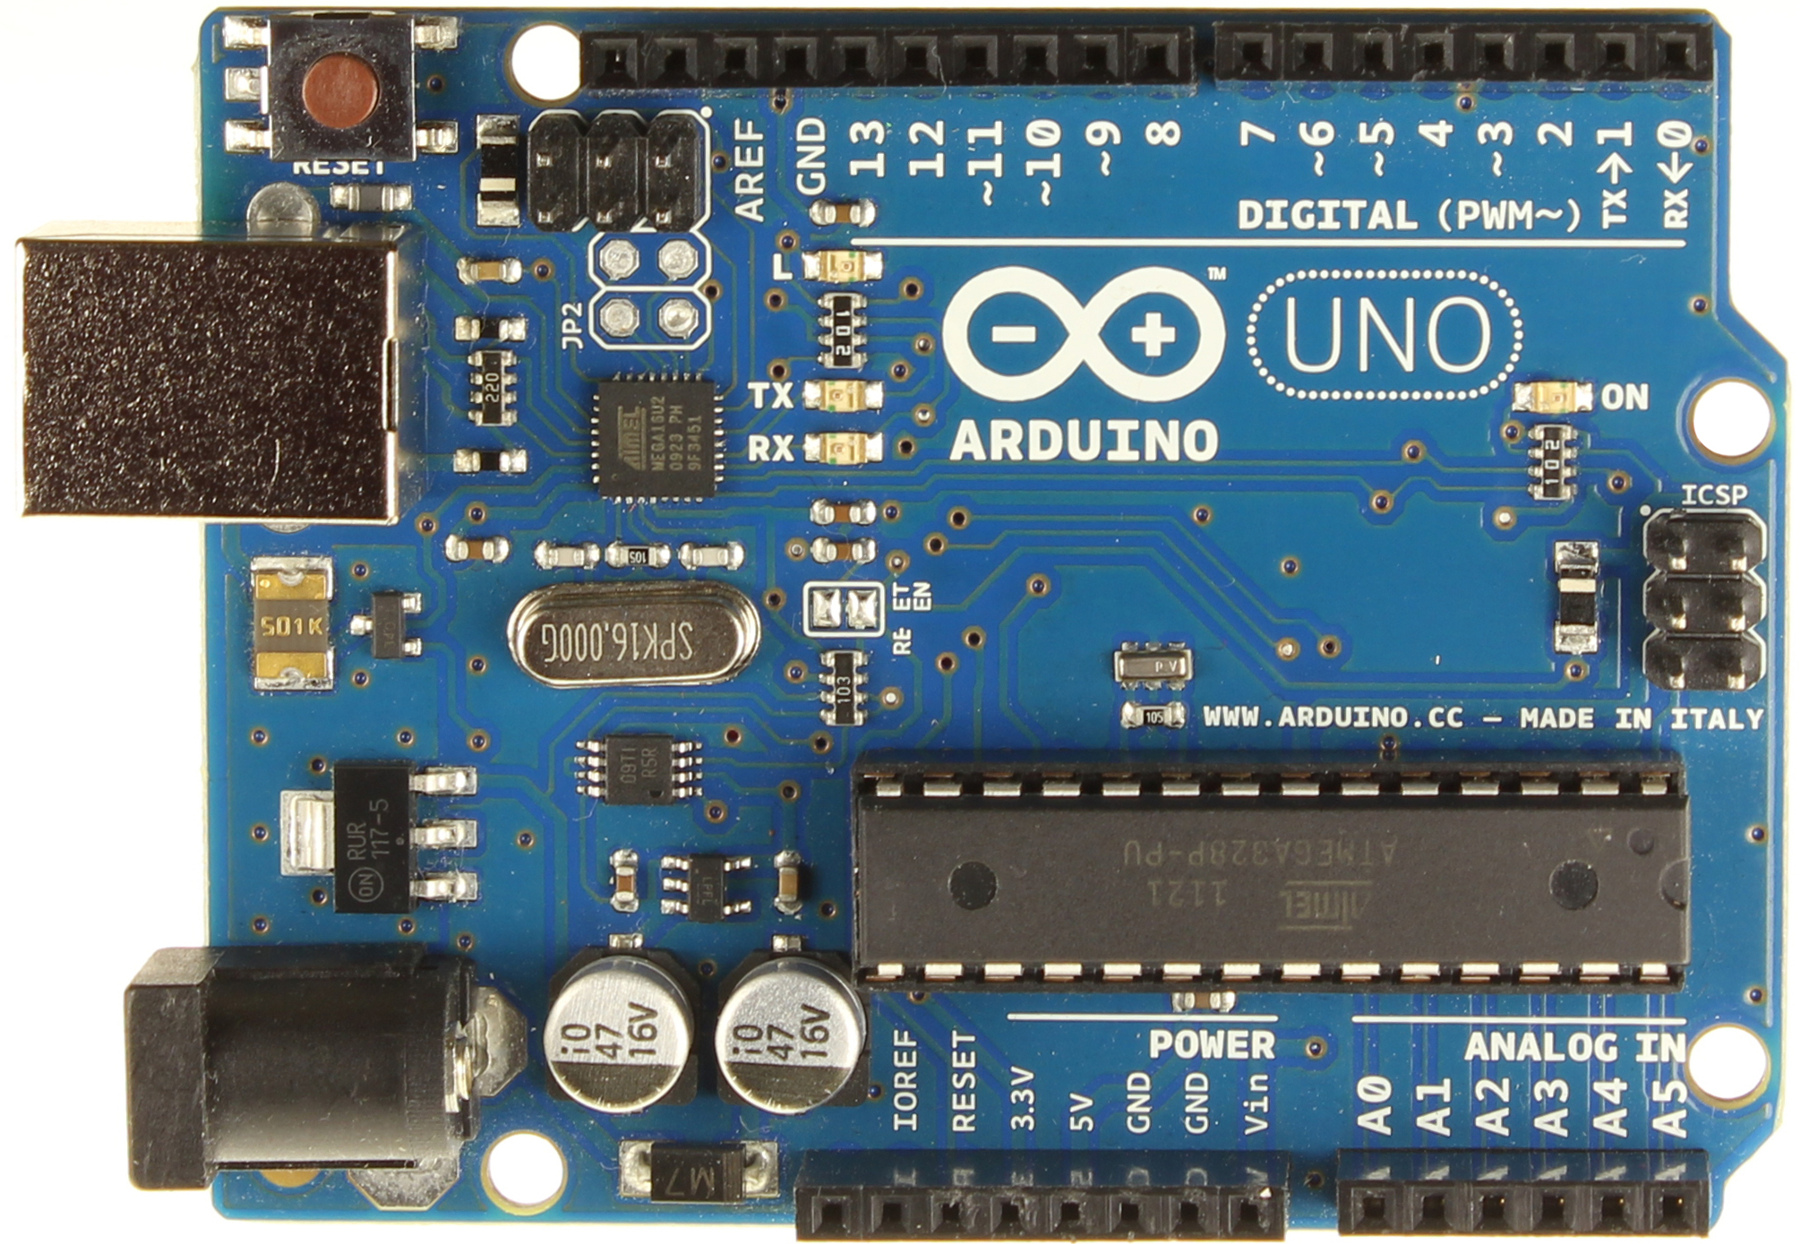
\includegraphics[scale=0.1,keepaspectratio=true]{./imagenes/arduino.jpg}
   % arduino.jpg: 1800x1244 pixel, 72dpi, 63.50x43.89 cm, bb=0 0 1800 1244
   \caption{Arduino}
   \label{figura:Arduino}
  \end{figure}

  \begin{figure}[htbp]
   \centering
   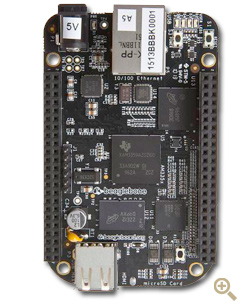
\includegraphics[scale=0.7,keepaspectratio=true]{./imagenes/beaglebone.jpg}
   % beaglebone.jpg: 247x306 pixel, 72dpi, 8.71x10.80 cm, bb=0 0 247 306
   \caption{BeagleBone}
   \label{figura:BeagleBone}
  \end{figure}

  \begin{figure}[htbp]
   \centering
   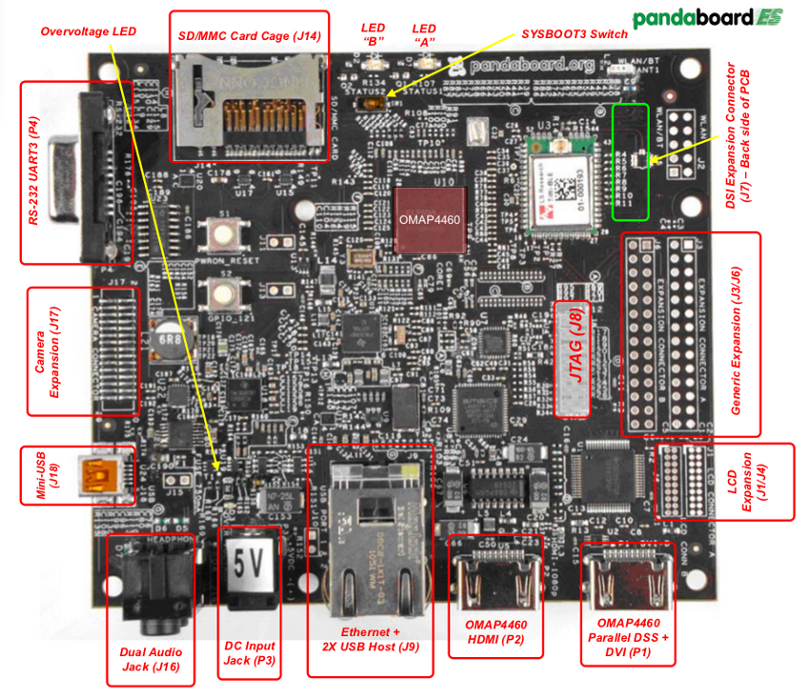
\includegraphics[scale=0.4,keepaspectratio=true]{./imagenes/pandaboard.png}
   % pandaboard.png: 810x699 pixel, 96dpi, 21.43x18.49 cm, bb=0 0 607 524
   \caption{PandaBoard}
   \label{figura:PandaBoard}
  \end{figure}

  \begin{figure}[htbp]
   \centering
   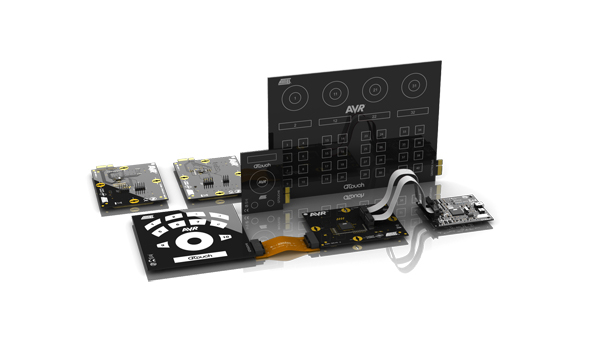
\includegraphics[scale=0.7,keepaspectratio=true]{./imagenes/qtouch.jpg}
   % qtouch.jpg: 600x338 pixel, 72dpi, 21.16x11.92 cm, bb=0 0 600 338
   \caption{Atmel QTouch}
   \label{figura:QTouch}
  \end{figure}

  \begin{figure}[htbp]
   \centering
   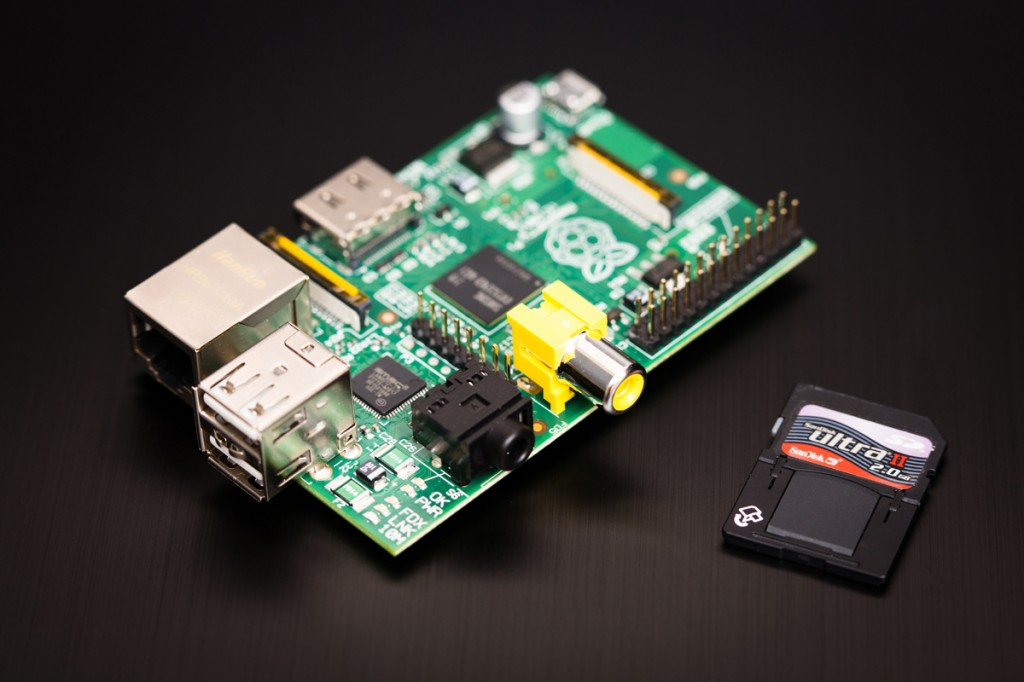
\includegraphics[scale=0.2,keepaspectratio=true]{./imagenes/raspberrypi.jpg}
   % raspberrypi.jpg: 1024x682 pixel, 72dpi, 36.12x24.06 cm, bb=0 0 1024 682
   \caption{Raspberry Pi}
   \label{figura:RaspberryPi}
  \end{figure}

  Tendo en conta os parámetros analizados e os requisitos do proxecto,
  determinouse que a plataforma Arduino\footnote{Para máis información sobre
  dita plataforma, consúltese o apéndice \ref{chap:arduino}.} ofrecía a mellor
  solución. \\

  Unha vez escollida a plataforma, había que, en base ó \textit{Prototipo 1},
  decidir qué compoñentes se necesitaban e cómo conectalos, é dicir, un deseño
  hardware inicial básico. \\

  A mellor maneira de coñecer as distintas posibilidades existentes era visitar
  a sección de hardware da páxina oficial de Arduino \cite{Arduino}, a tenda do
  maior fabricante de compoñentes para Arduino, de nome \textit{SparkFun}
  \cite{SparkFun} e as páxinas das dúas tendas oficiais principais dispoñibles
  en España, \textit{BricoGeek} \cite{BricoGeek} e \textit{Cooking Hacks}
  \cite{CookingHacks}. \\

  Para intentar acotar o hardware necesario, fíxose uso do
  \textit{Prototipo 1}, que constaba de tres seccións ben diferenciadas:

  \begin{itemize}
   \item Sensor de presión.
   \item Sensores capacitivos.
   \item Sistemas de recepción, procesamento, almacenamento, transmisión e
         alimentación.
  \end{itemize}

  Para cada unha destas seccións precisaba de un ou varios compoñentes, polo
  que se abordaron por partes. \\

  No tocante á primeira sección, precisábase dun sensor de presión que cumprise
  coas seguintes características:

  \begin{itemize}
   \item De dimensións moi reducidas.
   \item Que empregase un protocolo que non tivera problemas coas distancias.
   \item Cunha boa sensibilidade e que traballe con valores de presión
         elevados.
   \item De baixo consumo.
   \item Cun tempo de resposta moi pequeno.
   \item Tamén estaría ben que fose somerxible (aínda que isto é solventable).
  \end{itemize}

  Como sobre sensores non hai información na páxina oficial de Arduino, tocou
  buscar na páxina de SparkFun, na que se pode ver que a mellor opción
  dispoñible era o \textit{BMP085} \cite{BMP085} (figura \ref{figura:BMP085}).
  Mirando tamén nas tendas españolas, estaba tamén dispoñible. \\

  Ademais da súa distribución en territorio nacional, o deseño da placa de
  SparkFun facilita moito o traballo con el en sistemas modulares, de
  prototipado rápido e onde non exista posibilidade de soldar compoñentes
  SMD/BGA facilmente. \\

  Fixándose na súa folla de especificacións, vese que conta coas seguintes
  características:

  \begin{itemize}
   \item Dimensións: 16,5 x 16,5 mm.
   \item Consumo: 5 uA (máx).
   \item Precisión: 300 a 1100 hPa (9000 m a -500 m) con baixo ruido: 0,03 hPa
         (0,25 m).
   \item Protocolo: I2C.
   \item Tempo de resposta: 7,5 ms (máx.).
  \end{itemize}

  \begin{figure}[htbp]
   \centering
   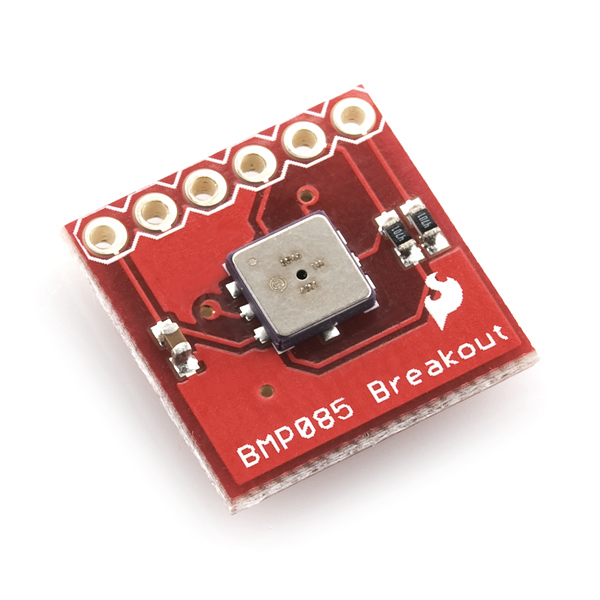
\includegraphics[keepaspectratio=true]{./imagenes/bmp085.jpg}
   % bmp085.jpg: 600x600 pixel, 300dpi, 5.08x5.08 cm, bb=0 0 144 144
   \caption{BMP085}
   \label{figura:BMP085}
  \end{figure}

  Polo que, cumprindo coas características solicitadas, deuse por bo e
  procedeuse a incorporalo ó deseño. \\

  Continuando coa segunda sección, precisábase dunha placa de sensores
  capacitivos que cumprise coas seguintes características:

  \begin{itemize}
   \item De dimensións reducidas.
   \item De baixo consumo.
   \item Con moi boa sensibilidade.
   \item Cun tempo de resposta moi pequeno.
   \item Alomenos con sitio para 9 sensores (número de buratos onde situar os
         dedos).
  \end{itemize}

  Estando no mesmo caso ca no anterior, volveu tocar ir á súa procura en
  SparkFun. E de todos os dispoñibles (que en realidade son variantes do
  mesmo), a que mellor se axustaba era a \textit{MPR121} \cite{MPR121}
  (figura \ref{figura:MPR121}). Fixándose na súa folla de especificacións, vese
  que conta coas seguintes características:

  \begin{itemize}
   \item Dimensións: 20 mm x 30 mm.
   \item Consumo: 29 uA (máx).
   \item Tempo de resposta: 1 ms a 128 ms (configurable en potencias de 2).
   \item Sensores: 12.
  \end{itemize}

  \begin{figure}[htbp]
   \centering
   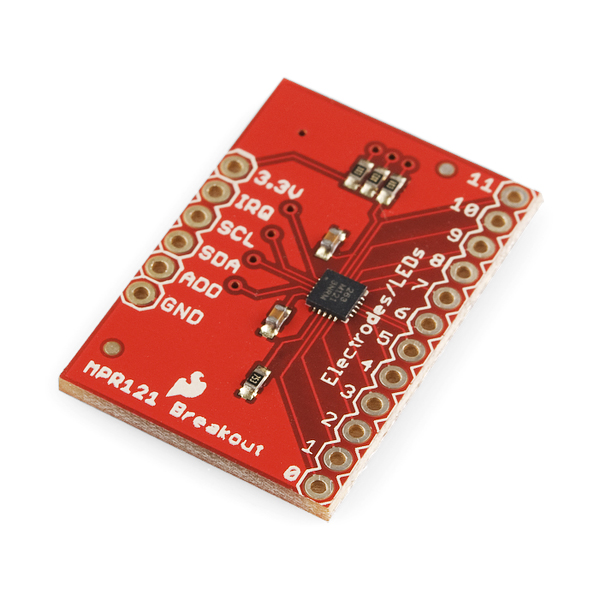
\includegraphics[keepaspectratio=true]{./imagenes/mpr121.jpg}
   % mpr121.jpg: 600x600 pixel, 300dpi, 5.08x5.08 cm, bb=0 0 144 144
   \caption{MPR121}
   \label{figura:MPR121}
  \end{figure}

  Polo que, cumprindo coas características solicitadas, deuse por boa e
  procedeuse a incorporala ó deseño. \\

  E rematando pola terceira sección, precisábase dun sistema que puidera:

  \begin{itemize}
   \item Recibir, procesar e transmitir (sen fíos) os sinais dos periféricos.
   \item Almacenar as configuracións.
   \item Que fose autónomo.
   \item De dimensións reducidas.
   \item De baixo consumo.
  \end{itemize}

  Dadas estas características, o que procedía era buscar unha placa base
  Arduino que cumprise coa maioría delas. Mirando, esta vez si, na páxina
  oficial, a que máis se axustaba era a Arduino Fio \cite{ArduinoFio} (figura
  \ref{figura:ArduinoFio}). Entre as súas características:

  \begin{itemize}
   \item Microcontrolador ATmega328P (8 Mhz, 3.3V).
   \item Comunicación mediante módulos Xbee.
   \item Soporta varios protocolos: Serie, I2C e SPI.
   \item Conexión para unha batería de Polímero Litio (recargable a través do
         miniUSB).
   \item Dimensións: 28 mm x 66 mm.
  \end{itemize}

  \begin{figure}[htbp]
   \centering
   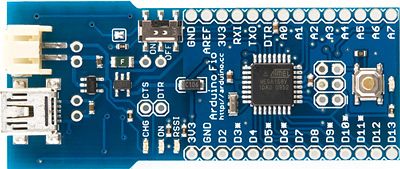
\includegraphics[scale=0.6,keepaspectratio=true]{./imagenes/arduino-fio.jpg}
   % arduino-fio.jpg: 400x169 pixel, 72dpi, 14.11x5.96 cm, bb=0 0 400 169
   \caption{Arduino Fio}
   \label{figura:ArduinoFio}
  \end{figure}

  Con respecto ós compoñentes que xa tiñamos, conta con soporte para I2C, polo
  que son perfectamente compatibles. \\

  O máis salientable quizáis sexa a comunicación sen fíos mediante
  \textit{XBee}\footnote{Para máis información sobre dita tecnoloxía consúltese
  o apéndice \ref{chap:xbee}.} \cite{Xbee}. Para o caso que nos compete,
  precisábase un módulo \textit{XBee} (non incluido coa placa
  \textit{Arduino Fio}) de pouca potencia (polo tanto menor consumo) e que
  permitise topoloxía de rede en estrela (pois o receptor tiña que permitir a
  conexión de varios punteiros simultaneamente). Entre os módulos dispoñibles
  na páxina do fabricante, o máis axeitado é o \textit{XBee ZB} \cite{XbeeZB}
  (figura \ref{figura:XBeeZB}):

  \begin{itemize}
   \item Protocolo: ZigBee (baseado en 802.15.4).
   \item Banda de transmisión: 2,4 GHz.
   \item Potencia de saída: 1,25/2 mW.
   \item Alcance: 120 m.
   \item Velocidade de transmisión: 250 Kbps.
   \item Consumo: 38 mA / \verb|<| 1 uA.
  \end{itemize}

  \begin{figure}[htbp]
   \centering
   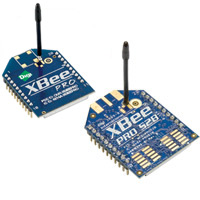
\includegraphics[scale=0.6,keepaspectratio=true]{./imagenes/xbee-zb.jpg}
   % xbee-zb.jpg: 200x200 pixel, 72dpi, 7.06x7.06 cm, bb=0 0 200 200
   \caption{XBee ZB}
   \label{figura:XBeeZB}
  \end{figure}

  Pero, ¿por que empregar \textit{XBee} e non outras tecnoloxías coma
  \textit{Bluetooth}\footnote{Versión inferior á 4.0. No momento de atacar esta
  parte non existían shields para Arduino con soporte para
  \textit{Bluetooth Low Energy} (BLE). As primeiras referencias datan de
  outubro de 2013.} ou
  \textit{WiFi}\footnote{Estándares IEEE 802.11a/b/g/n.}? Pois porque:

  \begin{itemize}
   \item Consume moito menos ca calquera das outras dúas tecnoloxía.
         \textit{XBee} ten un consumo de 30 mA transmitindo e 3 uA en repouso,
         fronte ós 40 mA transmitindo e 0,2 mA en repouso de \textit{Bluetooth}
         \cite{ZigBee}. Fronte á \textit{WiFi} pasa exactamente o mesmo.
   \item A velocidade de transmisión é superior á de \textit{Bluetooth}
         (115 Kbps, que é a velocidade á que poden chegar os módulos existentes
         para \textit{Arduino} a través de conexión por porto serie
         \cite{ArduinoBluetooth}).
   \item Ante a mesma potencia de saída, ten moito máis alcance ca calquera das
         outras dúas: 1 m para \textit{Bluetooth} \cite{Bluetooth} e 14 m para
         \textit{WiFi} \cite{WiFi}.
   \item A modo de resumo, aquí \cite{ComparativaZigBee} hai unha boa
         comparativa.
  \end{itemize}

  Ben, a estas alturas estaba solucionado o tema do emisor, pero seguía
  faltando o receptor. Ningún equipo existente no mercado xeral conta a día de
  hoxe con conexión \textit{XBee} integrada de serie, polo que foi preciso
  construír tamén un receptor. \\

  O primeiro que se precisaba era outro módulo \textit{XBee} exactamente igual
  para o receptor. Se non son exactamente iguais, a comunicación punto a punto
  non é posible \cite{ComunicacionXBee}. A priori, a conexión punto a punto non
  era unha necesidade, pero mellor ter a opción por se era necesaria a
  posteriori. \\

  E dito receptor había que conectalo a unha placa que nos permitise á súa vez
  conectalo a un equipo a través dalgún porto. \\

  O normal para un dispositivo MIDI sería empregar un porto MIDI (figura
  \ref{figura:WikipediaPortosMIDI}). Sen embargo, dito porto está actualmente
  en desuso, dada a súa aparatosidade e polo tanto a súa difícil integración en
  dispositivos de dimensións reducidas. Aínda que sigue sendo unha opción
  minoritaria en interfaces de audio de alta gama para ordenadores de
  sobremesa. Actualmente, as casas máis importantes de controladores hardware
  MIDI (\textit{Yamaha} e \textit{Roland}, principalmente) están a substituír
  (ou complementar) dita conexión por un porto USB (facilmente contrastable na
  folla de especificacións de calquera dos seus teclados actuais, por exemplo). \\

  É certo que existen placas complementarias para \textit{Arduino} con porto
  MIDI, coma esta \cite{SparkFunMIDI} (figura \ref{figura:SparkFunMIDI}), por
  exemplo, pero desbotouse esta opción en favor do novo estándar de facto do
  mercado, o USB. \\

  \begin{figure}[htbp]
   \centering
   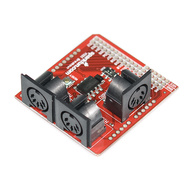
\includegraphics[scale=3.0,keepaspectratio=true]{./imagenes/sparkfun-midi.jpg}
   % sparkfun-midi.jpg: 188x188 pixel, 300dpi, 1.59x1.59 cm, bb=0 0 45 45
   \caption{MIDI Breakout}
   \label{figura:SparkFunMIDI}
  \end{figure}

  Novamente, voltando á páxina de \textit{SparkFun}, atopamos o
  \textit{XBee Explorer USB} \cite{XBeeExplorer} (figura
  \ref{figura:XBeeExplorer}) como a opción máis sinxela. Simplemente montar e
   enchufar. \\

  \begin{figure}[htbp]
   \centering
   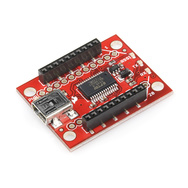
\includegraphics[scale=3.0,keepaspectratio=true]{./imagenes/xbee-explorer.jpg}
   % xbee-explorer.jpg: 188x188 pixel, 300dpi, 1.59x1.59 cm, bb=0 0 45 45
   \caption{XBee Explorer USB}
   \label{figura:XBeeExplorer}
  \end{figure}

  Pero esta opción plantexa un inconveniente con respecto a como o sería
  recoñecido o dispositivo por parte do equipo, polo que
  finalmente\footnote{Para máis información sobre cómo se solventou dito
  inconveniente, consúltese o capítulo \ref{chap:conclusiones}.} se optou
  por un empregar como base do receptor un \textit{Arduino Uno} (figura
  \ref{figura:ArduinoUno}) con firmware \textit{Moco} (figura
  \ref{figura:Moco}). \\

  \begin{figure}[htbp]
   \centering
   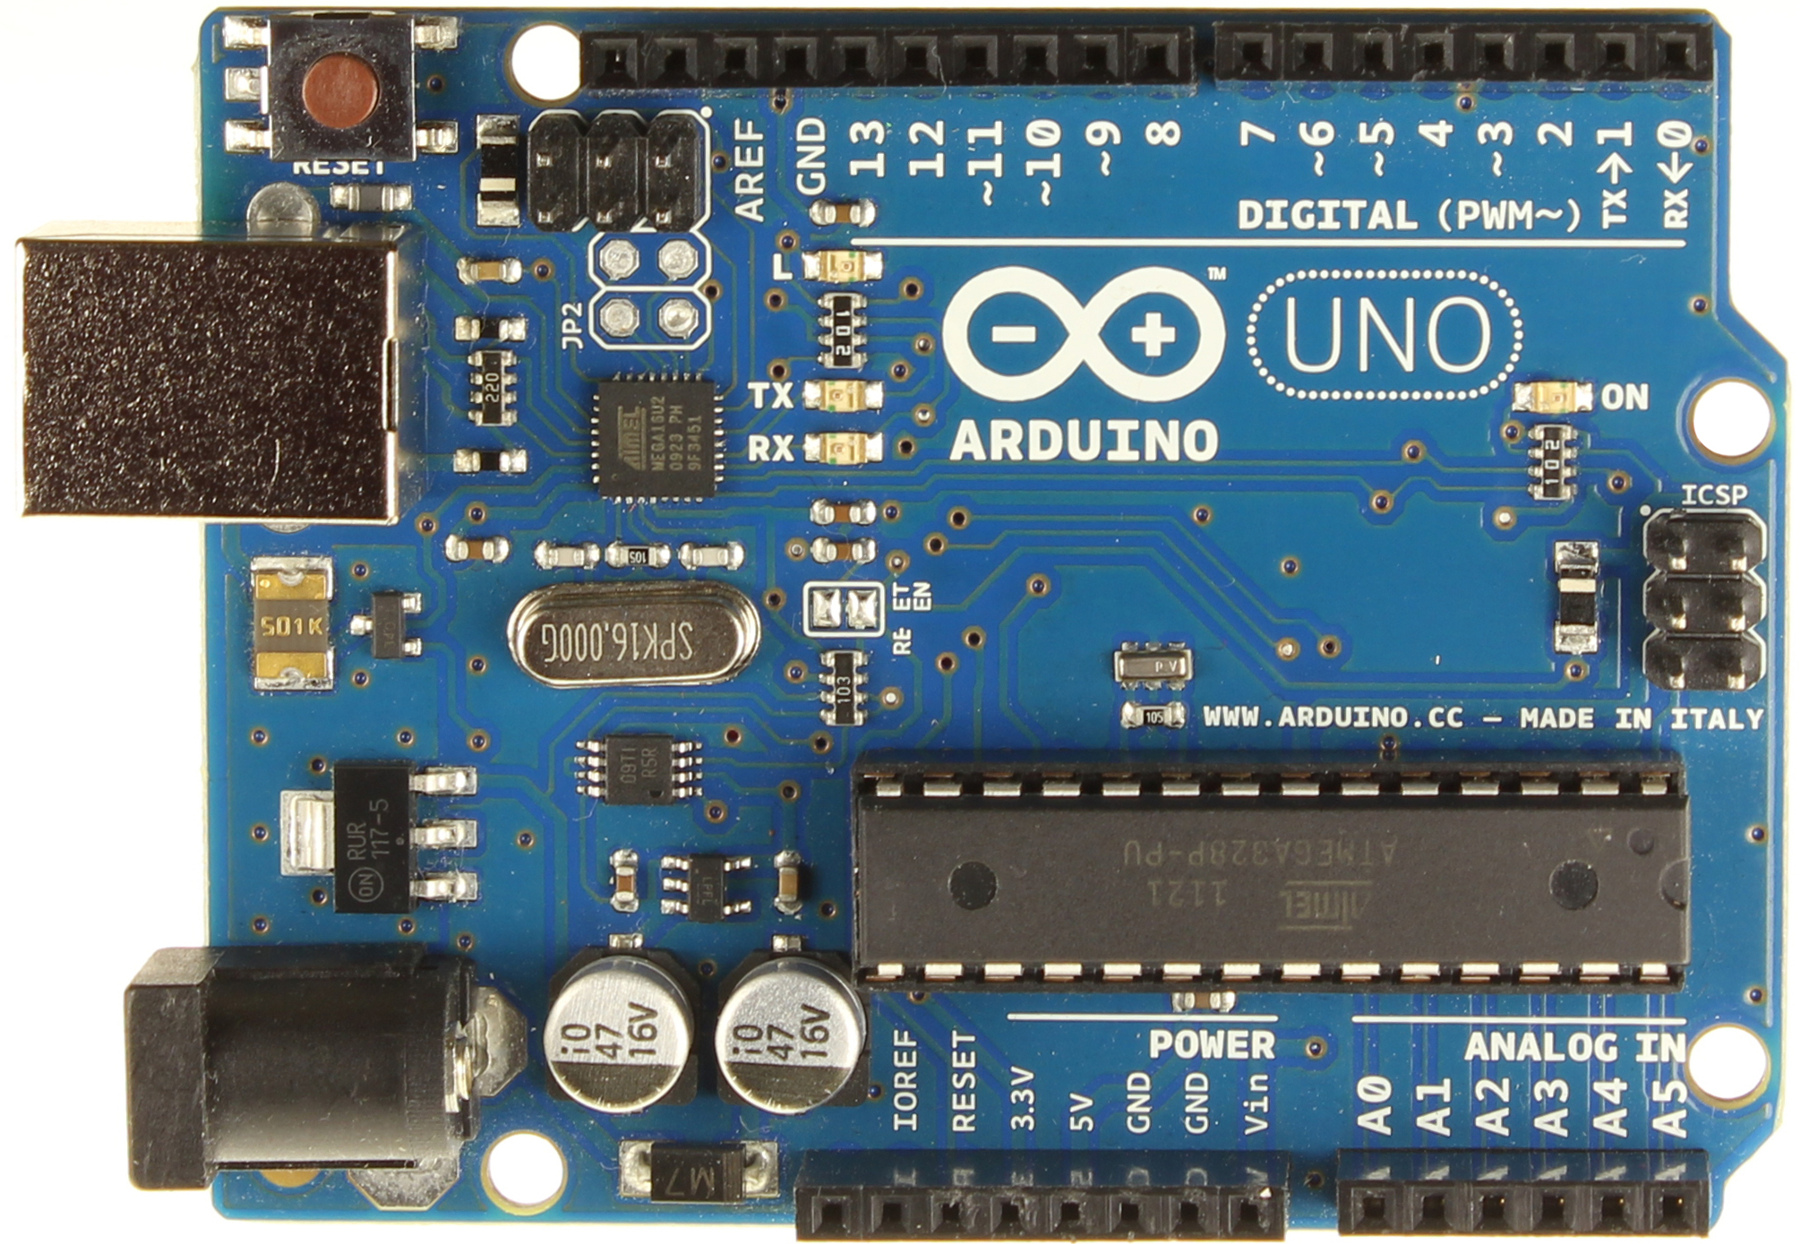
\includegraphics[scale=0.1,keepaspectratio=true]{./imagenes/arduino.jpg}
   % arduino.jpg: 1800x1244 pixel, 72dpi, 63.50x43.89 cm, bb=0 0 1800 1244
   \caption{Arduino}
   \label{figura:ArduinoUno}
  \end{figure}

  \begin{figure}[htbp]
   \centering
   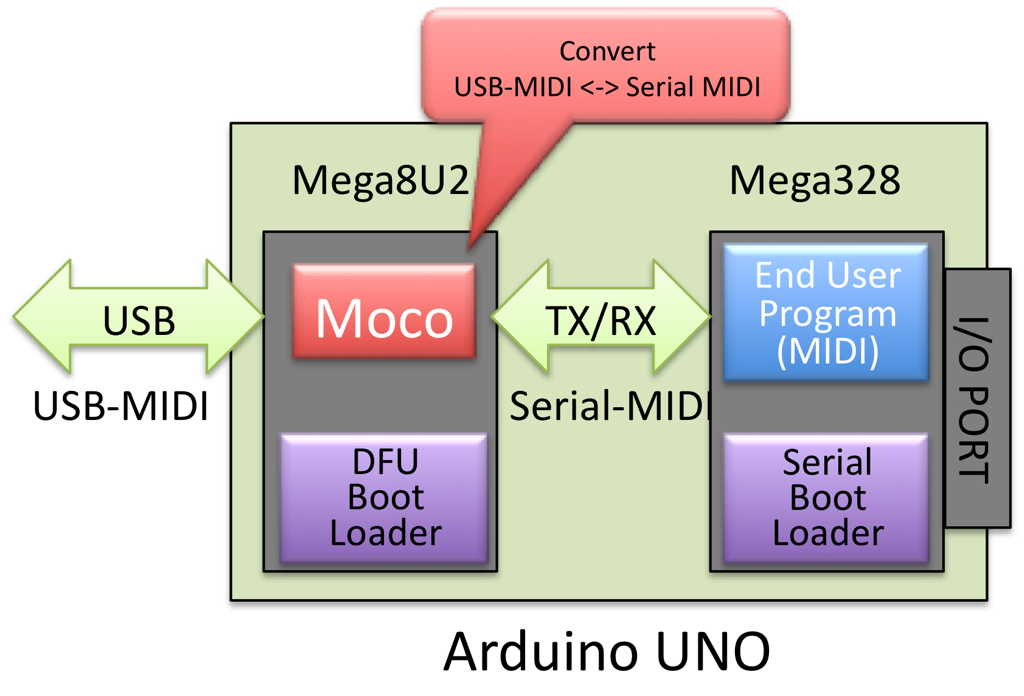
\includegraphics[scale=0.3,keepaspectratio=true]{./imagenes/moco.jpg}
   % moco.jpg: 1024x696 pixel, 72dpi, 36.12x24.55 cm, bb=0 0 1024 696
   \caption{Moco}
   \label{figura:Moco}
  \end{figure}

  Unha vez solucionado o problema de recoñecer o receptor coma dispositivo
  MIDI, quedaba atopar a maneira de conectar o módulo \textit{XBee} á placa
  \textit{Arduino Uno}. Dita placa non ten zócalo para módulos \textit{XBee}
  de serie, pero existen diversas solucións en forma de placas accesorias (ou
  \textit{shields}) que permiten conectar un módulo deste tipo. Entre as
  oficiais, contamos coa \textit{Arduino Wireless SD Shield}
  \cite{ArduinoWirelessShield} (figura \ref{figura:ArduinoWirelessShield}) e a
  \textit{Arduino Wireless Proto Shield} \cite{ArduinoWirelessProtoShield}
  (figura \ref{figura:ArduinoWirelessProtoShield}). As dúas son exactamente
  iguais coa excepción de que a primeira leva un lector de tarxetas de memoria
  de tipo SD e a segunda leva unha pequena zona de prototipado. Como resultaba
  máis interesante o lector de tarxetas para futuros usos, escolleuse a
  primeira.

  \begin{figure}[htbp]
   \centering
   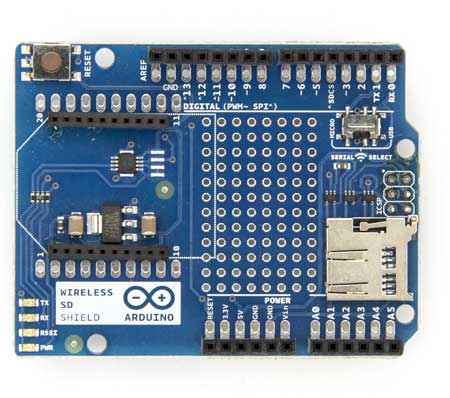
\includegraphics[scale=0.4,keepaspectratio=true]{./imagenes/arduino-wireless-shield.jpg}
   % arduino-wireless-shield.jpg: 450x398 pixel, 72dpi, 15.88x14.04 cm, bb=0 0 450 398
   \caption{Arduino Wireless SD Shield}
   \label{figura:ArduinoWirelessShield}
  \end{figure}

  \begin{figure}[htbp]
   \centering
   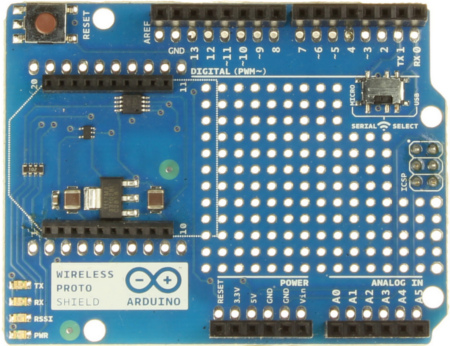
\includegraphics[scale=0.4,keepaspectratio=true]{./imagenes/arduino-wireless-proto-shield.jpg}
   % arduino-wireless-proto-shield.jpg: 450x346 pixel, 72dpi, 15.88x12.21 cm, bb=0 0 450 346
   \caption{Arduino Wireless Proto Shield}
   \label{figura:ArduinoWirelessProtoShield}
  \end{figure}

  E con isto quedaba listo o receptor, cuxas pezas se incorporaron ó deseño. \\

  Pero seguían quedando pendentes certas características do sistema embebido no
  punteiro: o almacenamento da configuración e a alimentación. \\

  Para o almacenamento da configuración, nun primeiro momento podíase chegar a
  pensar no lector de tarxetas do receptor, pero tendo en conta que cada
  punteiro ten a súa configuración independente e que un mesmo receptor pode
  ser usado por varios punteiros aleatorios simultáneamente, esta opción
  quedaba invalidada. \\

  Había que almacenar a información dentro do propio punteiro, pero ningún dos
  elementos incorporados previamente ó deseño (sensor de presión, placa de
  sensores capacitivos, Arduino Fio) contaba con zócalo para unha tarxeta de
  memoria, nin con ningunha placa accesoria que se puidese superpoñer á placa
  base do sistema. \\

  Tocou buscar nas páxinas de referencia se existía algunha placa de pequenas
  dimensións e baixo consumo que tivese coma función exclusiva a de lector de
  tarxetas de memoria. De entre todas as opcións existentes nas distintas
  páxinas de referencia, a mellor opción con diferencia era a
  \textit{MicroDrive G1} \cite{MicroDriveG1} (figura
  \ref{figura:MicroDriveG1}). Entre as súas características:

  \begin{itemize}
   \item Dimensións: 14,9 x 18,9 mm.
   \item Consumo: 25 mA.
   \item Almacenamento: tarxetas MicroSD de ata 4 GB ou MicroSD HC de tamaño
         superior.
   \item Formato: RAW ou FAT16.
   \item Protocolo: UART (serie).
  \end{itemize}

  \begin{figure}[htbp]
   \centering
   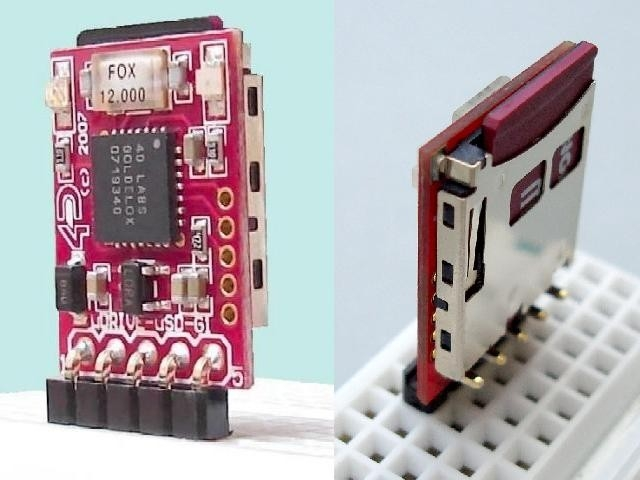
\includegraphics[scale=0.3,keepaspectratio=true]{./imagenes/microdrive-g1.jpg}
   % microdrive-g1.jpg: 640x480 pixel, 72dpi, 22.58x16.93 cm, bb=0 0 640 480
   \caption{MicroDrive G1}
   \label{figura:MicroDriveG1}
  \end{figure}

  Ten un consumo un pouco elevado, pero inferior ó do módulo \textit{XBee} e a
  calquera das outras alternativas no mercado, polo que é asumible. Ademais,
  emprega o protocolo Serie, polo que nos plantexaba un problema á hora de
  conectalo á placa \textit{Arduino Fio}, que só conta cun porto serie (RX/TX)
  que xa estaba a ser empregado polo módulo \textit{XBee}. Pero isto é
  facilmente solucionable mediante a biblioteca \textit{SoftwareSerial} de
  \textit{Arduino}, que nos permite xestionar múltiples periféricos con
  protocolo serie conectados a diferentes portos da mesma placa sen incrementar
  practicamente en nada a complexidade do código. \\

  Solventados os problemas, procedeuse a incorporar esta última placa ó deseño.
  Agora só quedaba buscar unha batería axeitada para a placa base, a
  \textit{Arduino Fio}. Debía de cumprir unha serie de requisitos:

  \begin{itemize}
   \item Ser de pequenas dimensións.
   \item Ser de Polímero Litio (LiPo).
   \item Ter bastante capacidade.
   \item Ter conector JST.
  \end{itemize}

  E entre todas as dispoñibles, a máis indicada era a \textit{LiPo 850 mAh}
  (figura \ref{figura:LiPo}) dispoñible en \textit{BricoGeek} \cite{LiPo}:

  \begin{itemize}
   \item Dimensións: 5,84 x 29,5 x 51 mm.
   \item Peso: 18,5 g.
   \item Tipo: 2C (3,7 V).
   \item Conector: JST.
   \item Material: LiPo.
  \end{itemize}

  \begin{figure}[htbp]
   \centering
   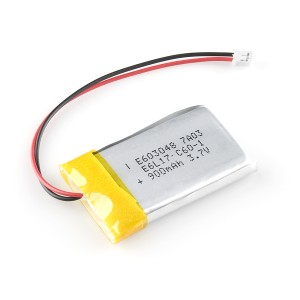
\includegraphics[scale=0.6,keepaspectratio=true]{./imagenes/lipo.jpg}
   % lipo.jpg: 300x300 pixel, 72dpi, 10.58x10.58 cm, bb=0 0 300 300
   \caption{Batería LiPo 850 mAh con conector JST}
   \label{figura:LiPo}
  \end{figure}

  Cumprindo coas características, incorporouse ó deseño. E con isto xa estaba
  case todo listo para poder pasar a realizar o \textbf{Prototipo 3}. \\

  Faltaba por escoller a ferramenta de deseño software apropiada para dita
  tarefa. Facendo unha busca rápida na rede sobre
  \textit{software de deseño hardware para Arduino}, damos con dúas solucións
  semellantes, pero ó mesmo tempo bastante diferentes: \textit{Eagle}
  \cite{Eagle} e \textit{Fritzing}\footnote{Para máis información sobre esta
  ferramenta, consúltese o apéndice \ref{chap:fritzing}.} \cite{Fritzing}.

  \begin{itemize}
   \item \textit{Eagle} é o sofware CAD propietario baixo cuxo formato se poñen
         dispoñibles os deseños oficiais de \textit{Arduino}. Aínda que na
         documentación diga que é sinxelo de usar, non o é tanto. Ten unha
         interface moi completa e bastante complexa que implica unha curva de
         aprendizaxe bastante lenta.
   \item \textit{Fritzing} é a contrapartida libre e sinxela a \textit{Eagle}.
         A interface é moito máis intuitiva, ademais de contar cunha base de
         datos de pezas de \textit{Arduino} (e periféricos das principais
         casas) bastante grande (o que aforra un traballo considerable á hora
         de facer os deseños) e cunha vista do resultado ``real'' coa que non
         conta \textit{Eagle} (moi interesante á hora de incluír os deseños na
         documentación).
  \end{itemize}

  Evidentemente, por cuestión de requisitos (e de principios) escolleremos
  sempre a versión libre (e máis sinxela) sobre a propietaria (sempre que a
  primeira funcione correctamente). \\

  A instalación da aplicación deu lugar a unha serie de incidencias, reflexadas
  no capítulo \ref{chap:conclusiones}. \\

  Solventadas ditas incidencias, puido comezarse co deseño. O primeiro foi
  buscar tódalas pezas na base de datos e incorporalas ó proxecto:

  \begin{itemize}
   \item A placa \textit{Arduino Fio}, non contaba expresamente co zócalo para
         o módulo \textit{XBee}. Isto é debido a que só se pode reflexar unha
         cara das pezas no software, polo que o módulo, que quedaba na outra
         cara, quedou sen reflexar. O autor da mesma podía ter optado por
         desdobrar a peza e reflexala, pero non o fixo. Por este motivo, a
         conexión do módulo XBee tivo que ser directa ós pines xenéricos da
         placa.
   \item A placa de sensores capacitivos \textit{MPR121} non estaba dispoñible
         na súa versión \textit{Breakout} pero si na versión \textit{Touch}. A
         única diferencia é que esta última incorpora varios electrodos xa na
         propia placa, polo que o seu tamaño é un pouco maior, pero non inflúe
         no deseño, pois conta coas mesmas conexións, polo que para un deseño
         ``non físico'' é equivalente.
   \item A placa de almacenamento \textit{MicroDrive G1} non estaba dispoñible
         na base de datos do software por ser dun fabricante menos coñecido.
         Afortunadamente, estaba dispoñible no apartado de contribucións do
         repositorio da aplicación \cite{FioContribucionsFritzing}. Unha vez
         descargada, intentouse incorporala ó proxecto, pero non foi posible,
         pois tiña algún tipo de erro (e por iso non estaba incluida na base de
         datos). O como se solucionou esta incidencia coméntase tamén no
         capítulo \ref{chap:conclusiones}.
  \end{itemize}

  Unha vez incorporadas todas as pezas ó proxecto, procedeuse a facer as
  conexións pertinentes mediante cable, previo estudo das follas de
  especificacións de cada peza (conexións, protocolos, etc.). Compre aclarar
  que moitos deses cables non aparecerán como tal no producto hardware final,
  dado que a maioría das pezas son ensamblables, pero esta característica non
  se pode reflexar na aplicación. A continuación expóñense as distintas vistas
  do deseño (figuras \ref{figura:Prototipo3HardwareBB} e
  \ref{figura:Prototipo3HardwareEsquema}).

  \begin{figure}[htbp]
   \centering
   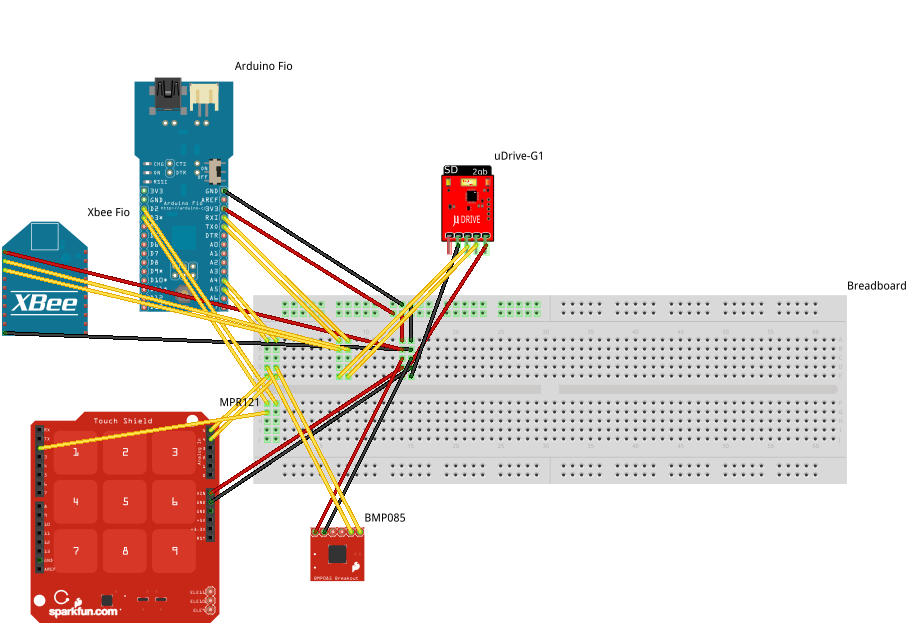
\includegraphics[scale=0.55,keepaspectratio=true]{./imagenes/prototipo3_bb_1.png}
   % prototipo3_bb_1.png: 918x639 pixel, 96dpi, 24.29x16.90 cm, bb=0 0 688 479
   \caption{Prototipo 3 hardware, emisor: vista real}
   \label{figura:Prototipo3HardwareBB1}
  \end{figure}

  \begin{figure}[htbp]
   \centering
   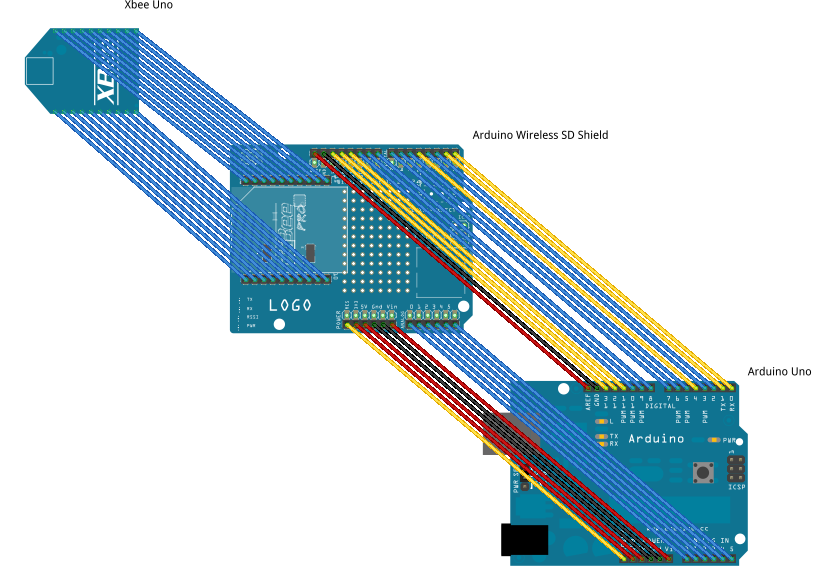
\includegraphics[scale=0.55,keepaspectratio=true]{./imagenes/prototipo3_bb_2.png}
   % prototipo3_bb_2.png: 827x588 pixel, 96dpi, 21.88x15.56 cm, bb=0 0 620 441
   \caption{Prototipo 3 hardware, receptor: vista real}
   \label{figura:Prototipo3HardwareBB2}
  \end{figure}

  \begin{figure}[htbp]
   \centering
   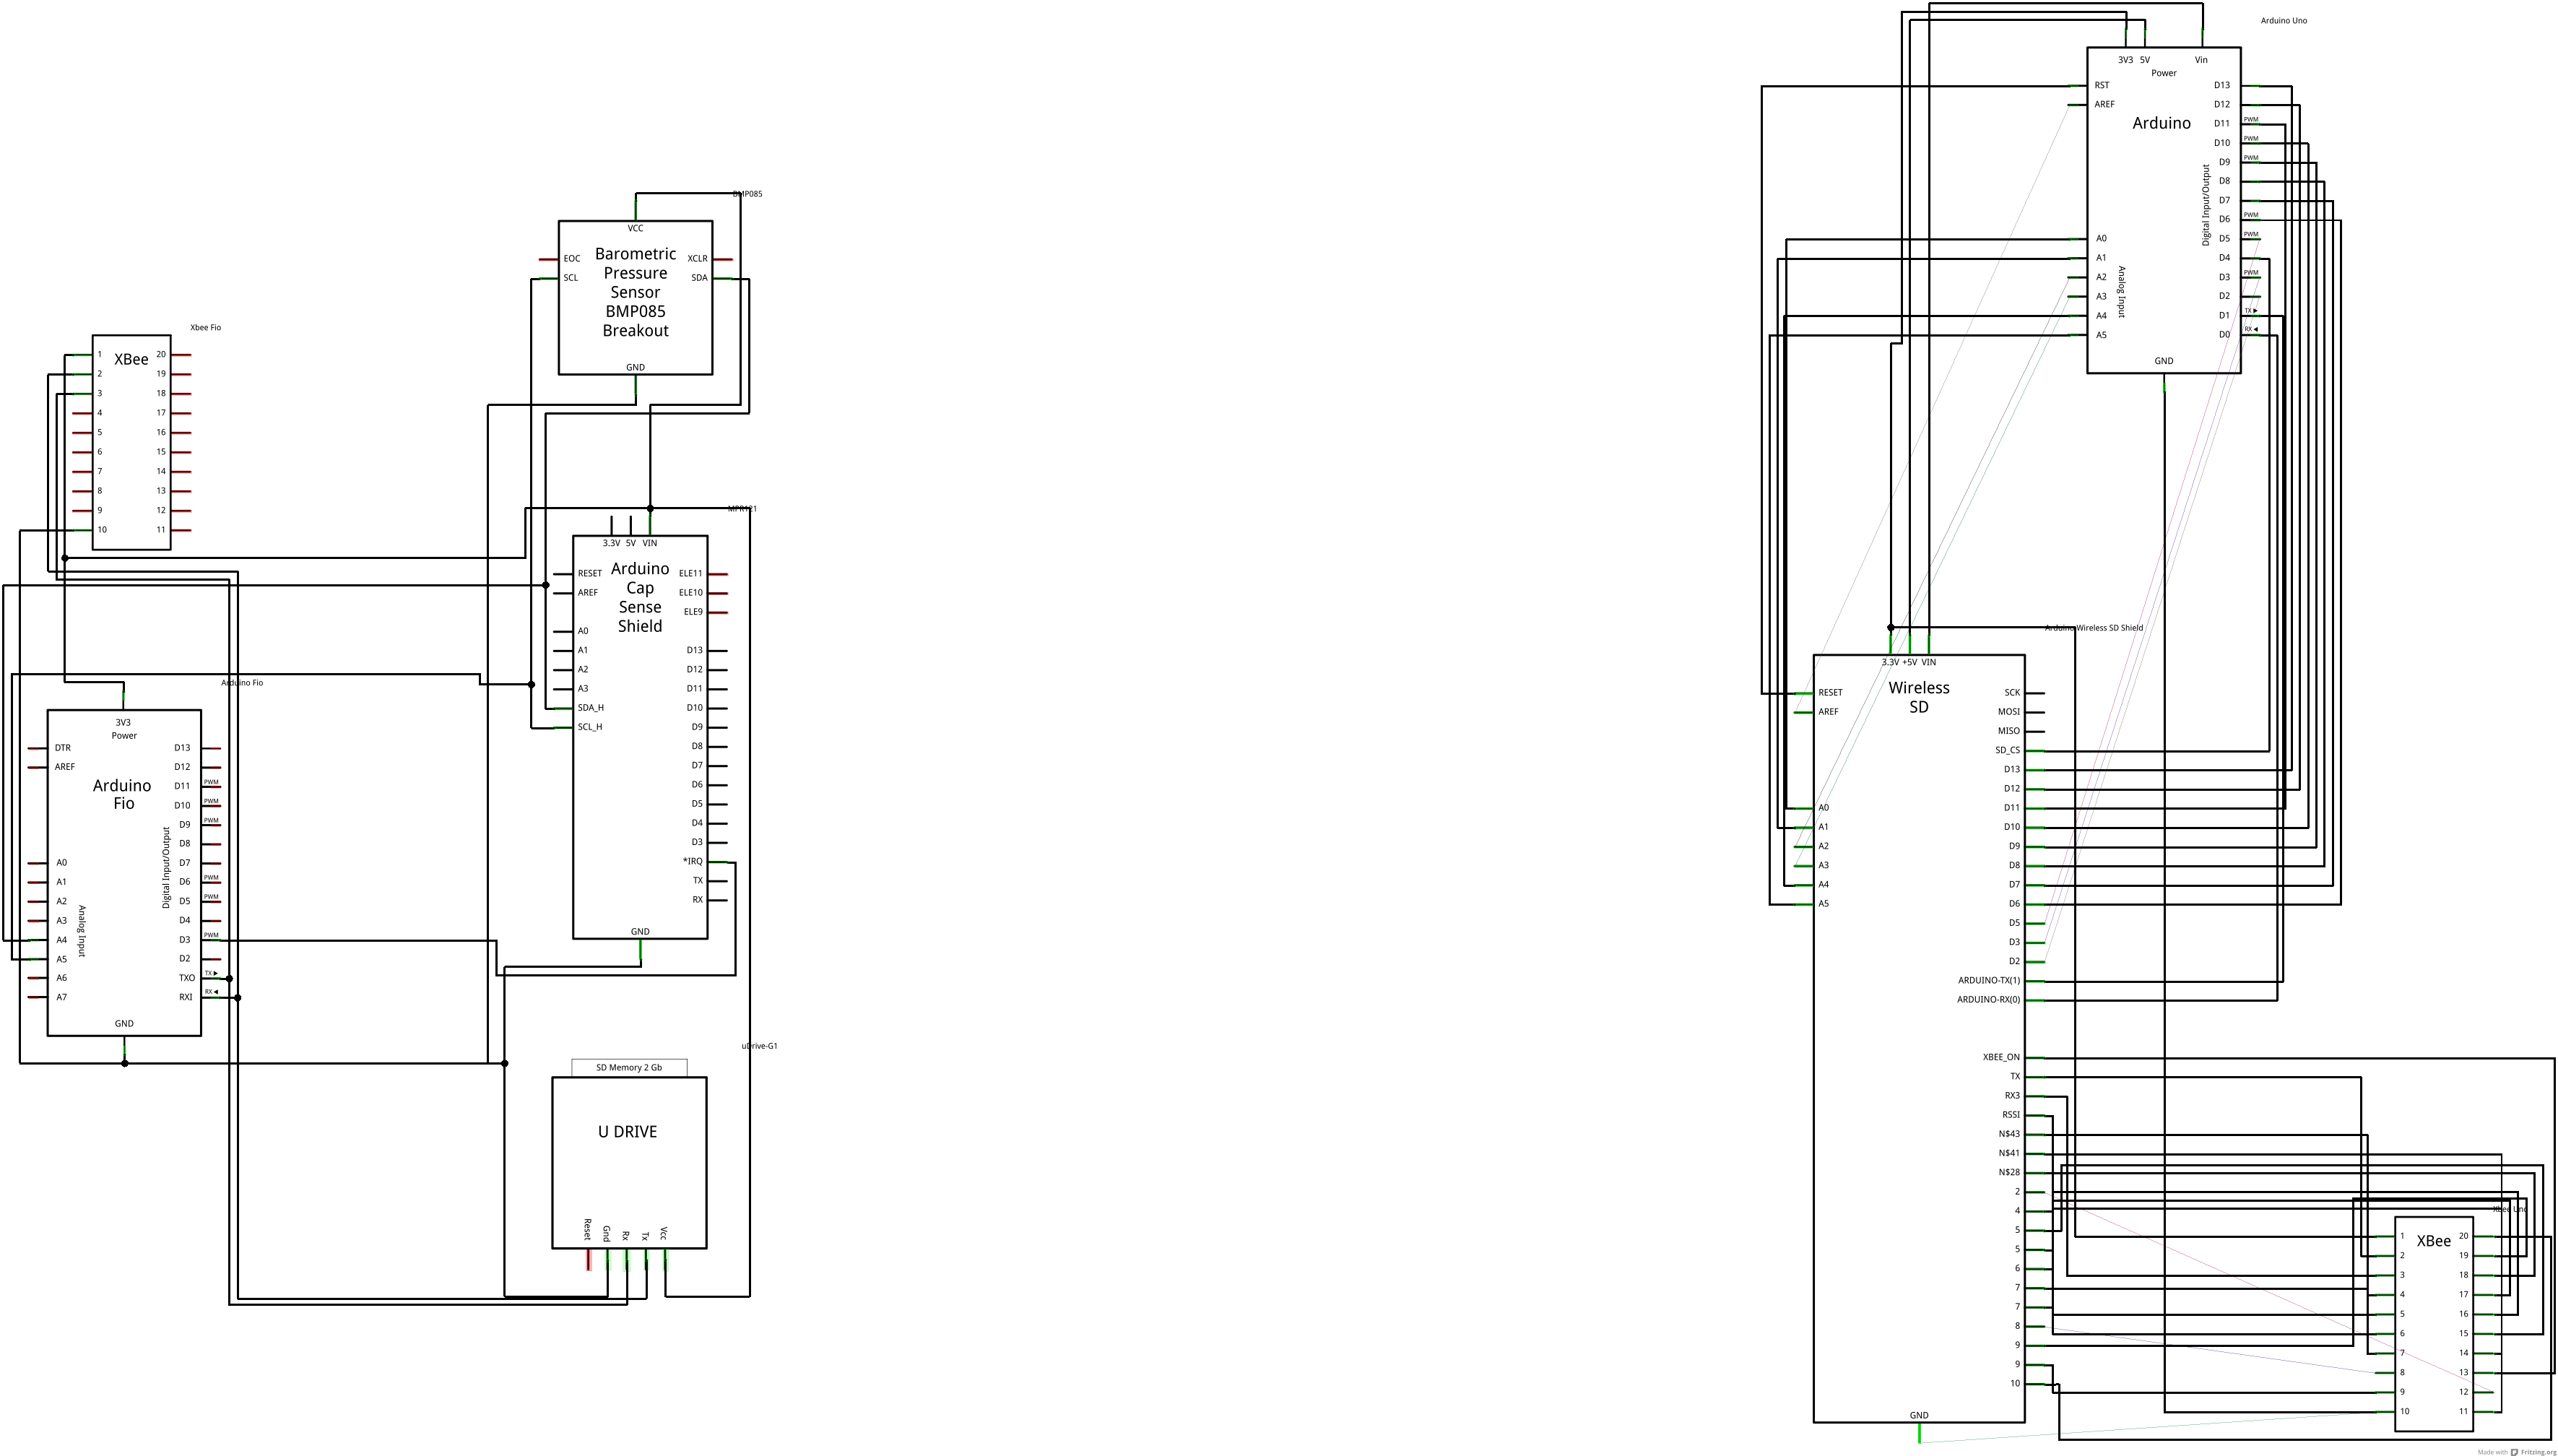
\includegraphics[scale=30.0,keepaspectratio=true]{./imagenes/prototipo3_esquema.png}
   % prototipo3_esquema.png: 3542x2016 pixel, 7742dpi, 1.16x0.66 cm, bb=0 0 33 19
   \caption{Prototipo 3 hardware: vista esquemática}
   \label{figura:Prototipo3HardwareEsquema}
  \end{figure}

  \subsubsection{Prototipo software}

  O \textit{Prototipo 3} na súa vertente software, é basicamente o
  \textit{Prototipo 2} con moi lixeiras modificacións:

  \begin{itemize}
   \item Axustáronse as referencias ás oitavas ós valores dados polo estándar
         americano de notación musical, que é o máis empregado.
   \item Incluíuse a opción de poder modificar a sensibilidade de tódolos
         sensores á vez, que aínda que estaba contemplada, pasárase por alto
         metela no despregable.
   \item Despois de rematar o \textit{Prototipo 3} na súa versión hardware,
         púidose comprobar que a placa de sensores capacitivos \textit{MPR121}
         conta con dous valores axustables, o de \textit{press} e o de
         \textit{release}, polo que se incluíu outro \textit{slider} na
         interface para poder controlar tamén este último a vontade.
  \end{itemize}

  Feitos todos estes pequenos cambios, o \textbf{Prototipo 3} software quedou
  como segue (figuras \ref{figura:Prototipo3Inicio} a 
  \ref{figura:Prototipo3Dixitacion}).

  \begin{figure}[htbp]
   \centering
   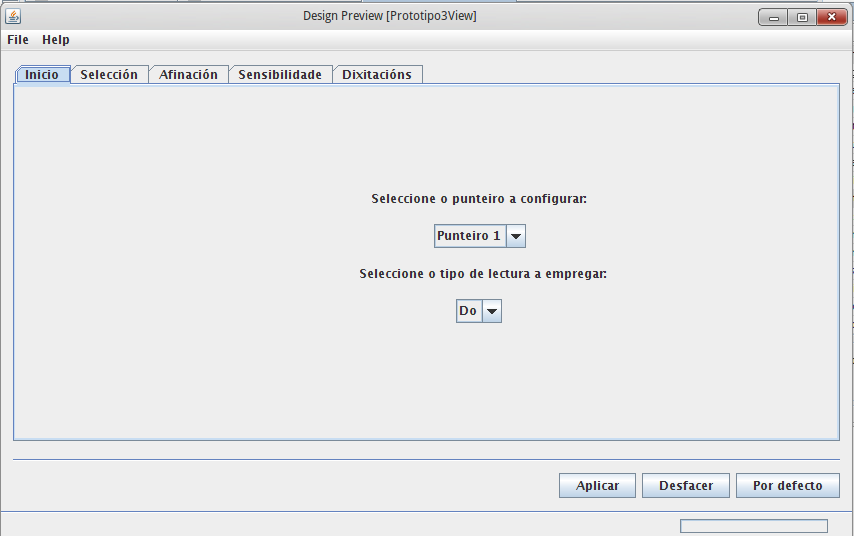
\includegraphics[scale=0.6,keepaspectratio=true]{./imagenes/prototipo3-1.png}
   % prototipo3-1.png: 854x536 pixel, 96dpi, 22.59x14.18 cm, bb=0 0 640 402
   \caption{Prototipo 3: pantalla de inicio}
   \label{figura:Prototipo3Inicio}
  \end{figure}

  \begin{figure}[htbp]
   \centering
   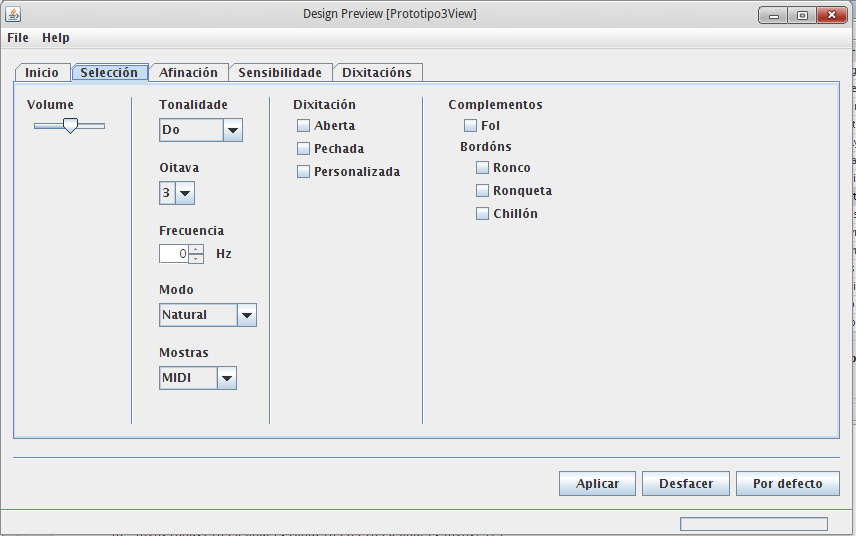
\includegraphics[scale=0.6,keepaspectratio=true]{./imagenes/prototipo3-2.png}
   % prototipo3-2.png: 856x536 pixel, 96dpi, 22.65x14.18 cm, bb=0 0 642 402
   \caption{Prototipo 3: pantalla de selección}
   \label{figura:Prototipo3Seleccion}
  \end{figure}

  \begin{figure}[htbp]
   \centering
   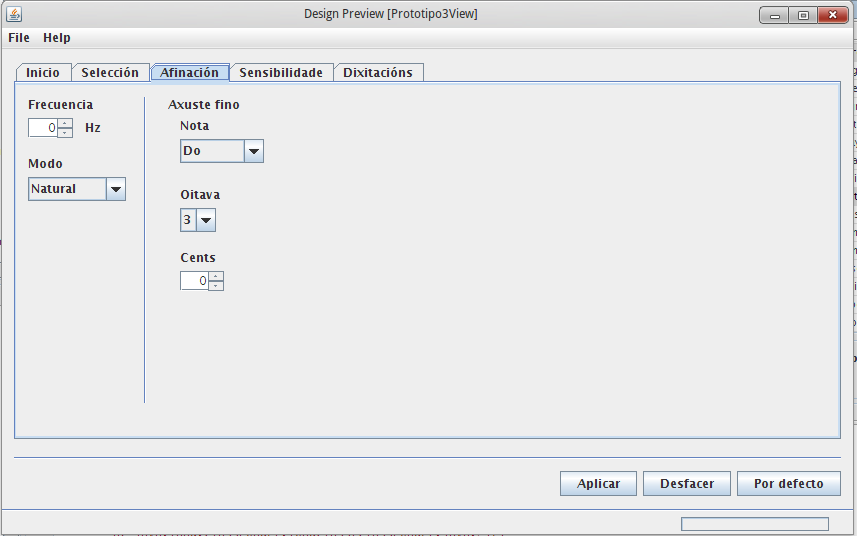
\includegraphics[scale=0.6,keepaspectratio=true]{./imagenes/prototipo3-3.png}
   % prototipo3-3.png: 857x536 pixel, 96dpi, 22.67x14.18 cm, bb=0 0 643 402
   \caption{Prototipo 3: pantalla de afinación}
   \label{figura:Prototipo3Afinacion}
  \end{figure}

  \begin{figure}[htbp]
   \centering
   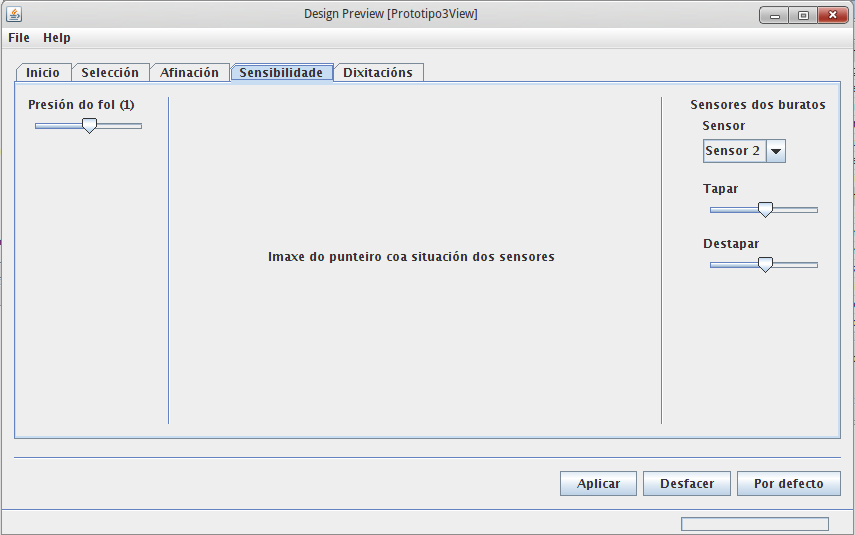
\includegraphics[scale=0.6,keepaspectratio=true]{./imagenes/prototipo3-4.png}
   % prototipo3-4.png: 855x535 pixel, 96dpi, 22.62x14.15 cm, bb=0 0 641 401
   \caption{Prototipo 3: pantalla de sensibilidade}
   \label{figura:Prototipo3Sensibilidade}
  \end{figure}

  \begin{figure}[htbp]
   \centering
   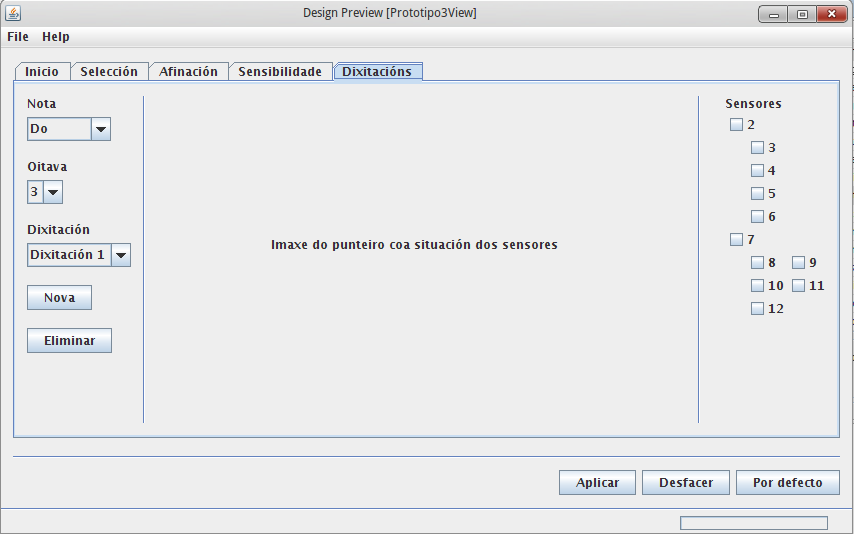
\includegraphics[scale=0.6,keepaspectratio=true]{./imagenes/prototipo3-5.png}
   % prototipo3-5.png: 854x534 pixel, 96dpi, 22.59x14.13 cm, bb=0 0 640 400
   \caption{Prototipo 3: pantalla de dixitación}
   \label{figura:Prototipo3Dixitacion}
  \end{figure}

\section{Desenvolvemento e validación do seguinte nivel do producto}

 \subsection{Simulacións, modelos e programas de proba}

 As probas a realizar neste nivel do producto dividíronse en dous grupos:

 \begin{itemize}
  \item Por unha banda, consistiron en verificar sobre o
        \textit{Prototipo 3 hardware} todos aqueles requisitos hardware
        aplicables ó mesmo recollidos na especificación de requisitos.
  \item Por outra, verificouse novamente o \textit{Prototipo 3 software} para
        que comprobar que os pequenos cambios introducidos non inducisen a unha
        inconformidade coa especificación de requisitos.
  \item E finalmente, verificouse contra a especificación de requisitos o
        deseño obtido a partir de ambos prototipos e validous o seu
        funcionamento atendendo ás funcionalidades solicitadas.
 \end{itemize}

 \subsection{Deseño do producto hardware e software}

  \subsubsection{Deseño do producto hardware}

  Contando xa cun deseño formal dende a fase de prototipado e solventados todos
  os pequenos problemas que se atoparon durante o desenvolvemento do mesmo,
  decidiuse empregar o propio \textit{Prototipo 3 hardware} coma deseño do
  producto hardware.

  \subsubsection{Deseño do producto software}

  Atendendo ó deseño dos prototipos anteriores, téñense dúas aplicacións ben
  diferenciadas:

  \begin{itemize}
   \item A aplicación embebida dentro do punteiro
         (\textit{Prototipo 3 hardware}), que se encarga de do control e
         configuración do hardware e de proporcionar as funcionalidades do
         mesmo.
   \item E a aplicación de escritorio, encargada da configuración tanto do
         punteiro coma do sintetizador.
  \end{itemize}

  Polo tanto, houbo que tratalas coma tal e realizar dous deseños
  independentes, pero ó mesmo tempo relacionados. O resultado ó que se chegou
  foi o da figura \ref{figura:DesenoAltoNivel}.

  \begin{figure}[htbp]
   \centering
   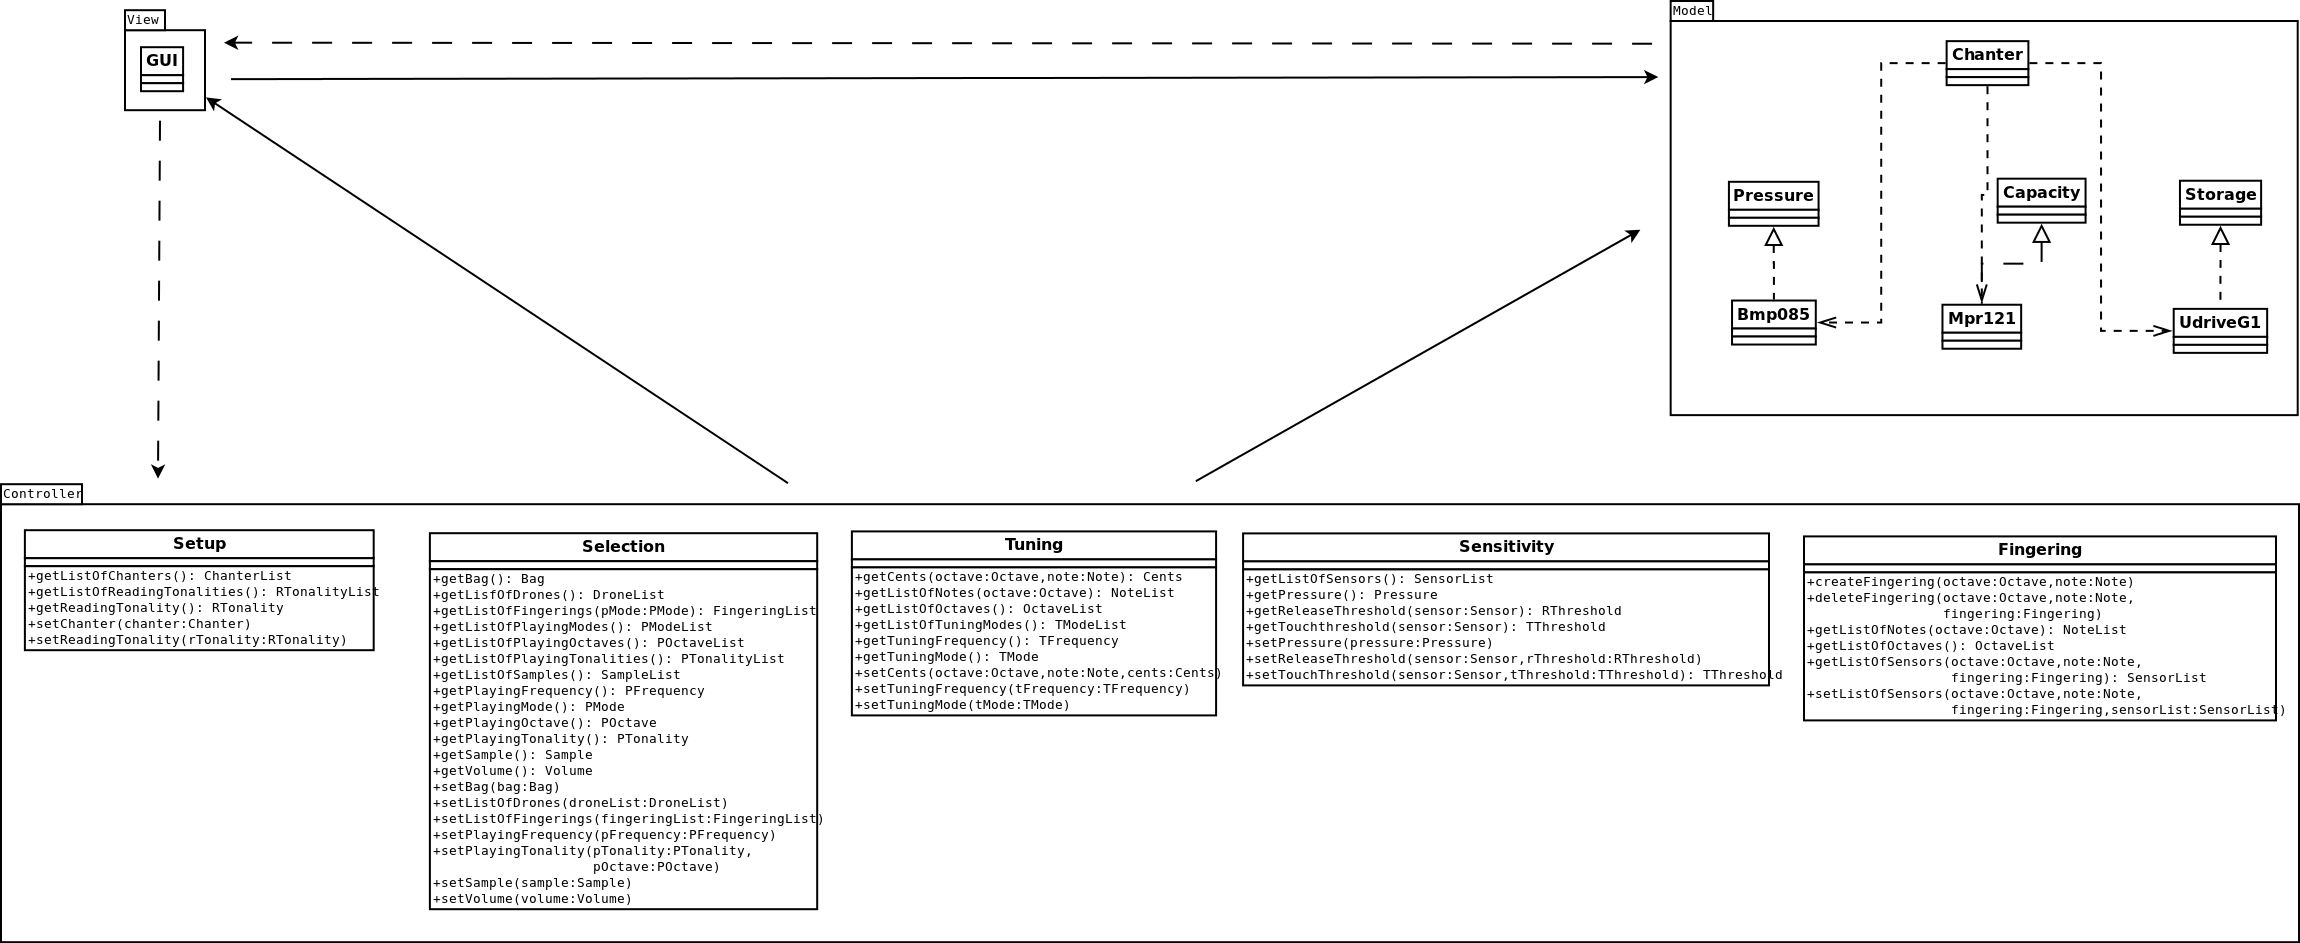
\includegraphics[scale=0.25,angle=90,keepaspectratio=true]{./imagenes/desenho-an.png}
   % desenho-an.png: 2300x943 pixel, 72dpi, 81.14x33.27 cm, bb=0 0 2300 943
   \caption{Deseño de alto nivel}
   \label{figura:DesenoAltoNivel}
  \end{figure}

  Como se pode apreciar, existe un patrón Modelo-Vista-Controlador, onde:

  \begin{itemize}
   \item A Vista correspóndese coa interface gráfica ou GUI.
   \item O Controlador é un conxunto de clases, agrupadas segundo a división en
         pestanas da interface gráfica e que inclúen tódalas funcións
         necesarias para o correcto funcionamento da Vista.
   \item O Modelo correspóndese coa aplicación embebida no punteiro. O deseño
         da mesma é un pouco peculiar, xa que nun principio non vai ser
         orientada a obxectos (aínda que podería, dada a versatilidade de
         Arduino), pois non aporta demasiado, como se pode comprobar no propio
         deseño; pero non deixa de ser unha maneira equivalente de representalo
         á hora de plasmalo en UML.
  \end{itemize}

  Así mesmo, cómpre lembrar que se trata dun deseño de alto nivel e, polo
  tanto, só se representaron as clases máis significativas. O que se pretende é
  dar unha noción básica do deseño da aplicación, facilitando a súa
  comprensión, evitando a complexidade dun deseño recargado de clases
  secundarias que pouco ou nada aportarían.

 \subsection{Verificación e validación do deseño}

 Realizadas as probas anteriormente definidas e verificados e validados os dous
 deseños previos, non se atoparon inconformidades, polo que se deron por bos e
 se continuou coa seguinte fase.

\section{Planificación da próxima fase ou ciclo}

 \subsection{Planificación do desenvolvemento}

 A continuación (figura \ref{figura:PlanificacionInicialDesenvolvemento})
 exponse a planificación inicial do ciclo de desenvolvemento. \\

 \begin{figure}[htbp]
  \centering
  %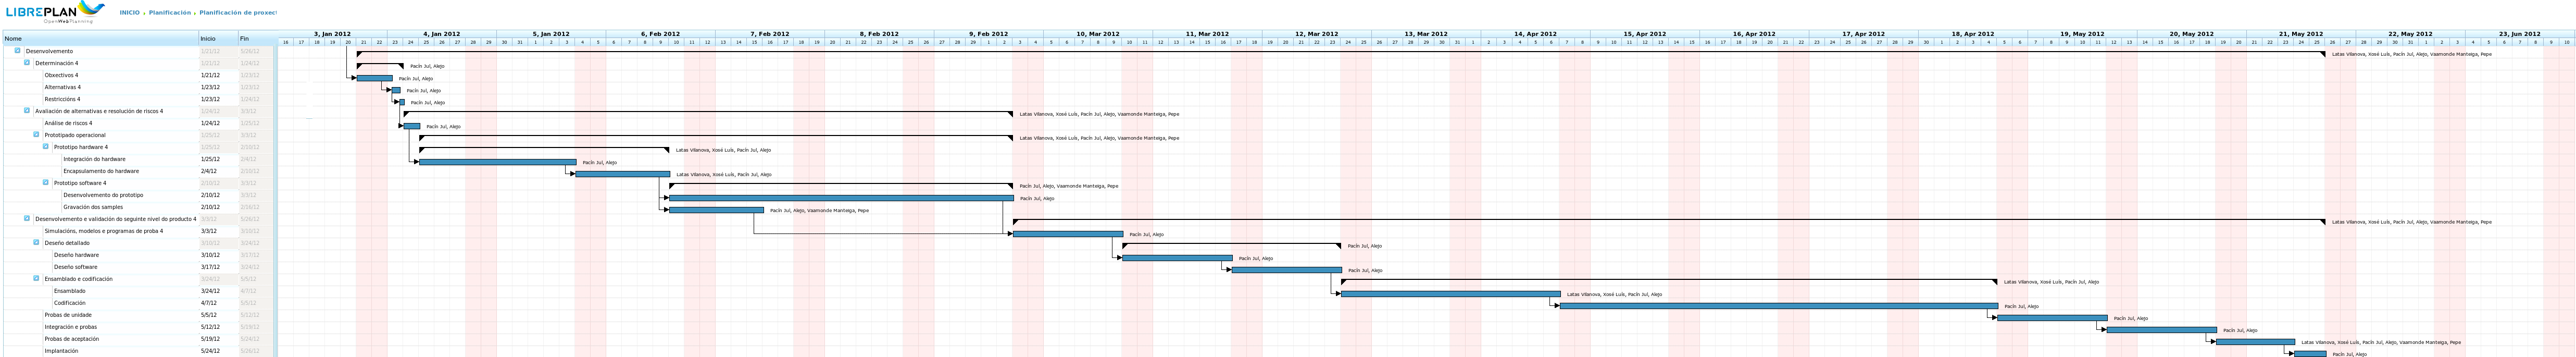
\includegraphics[scale=0.15,angle=90,keepaspectratio=true]{./imagenes/desenvolvemento.png}
  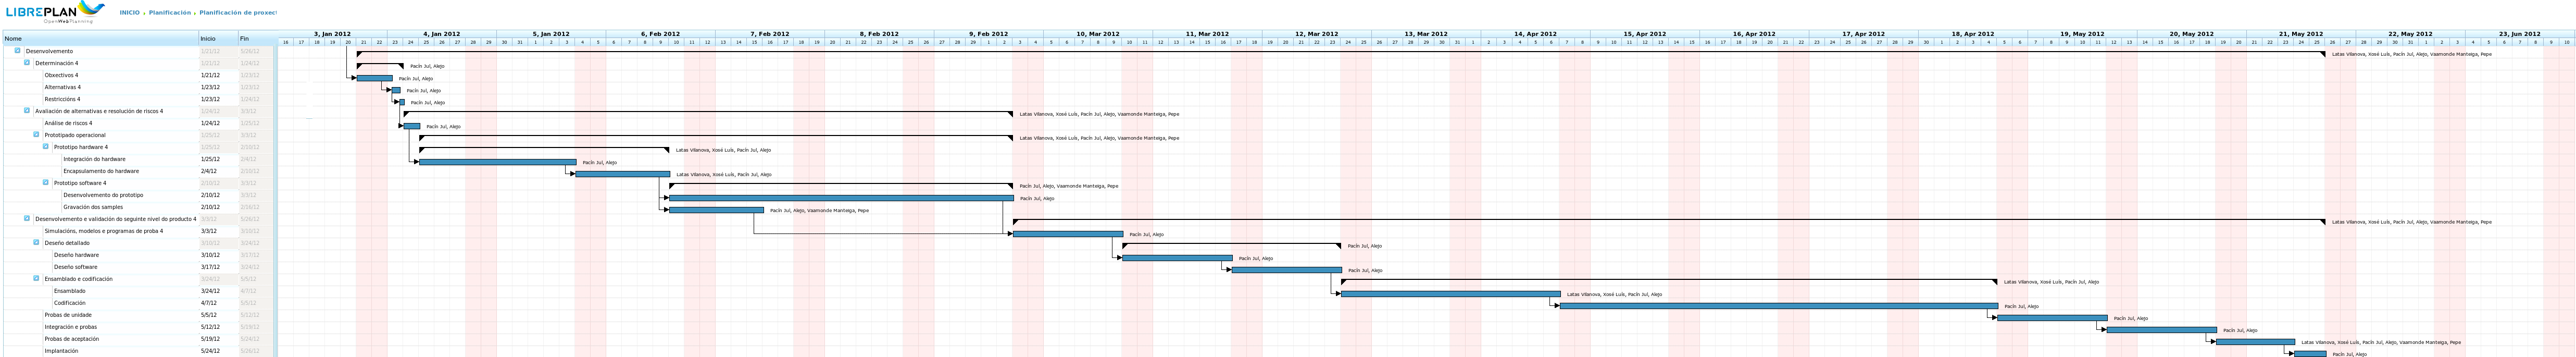
\includegraphics[trim=0 0 112cm 0,clip=true,scale=0.70,keepaspectratio=true]{./imagenes/desenvolvemento.png}
  % desenvolvemento.png: 4946x685 pixel, 100dpi, 125.63x17.40 cm, bb=0 0 3561 493
  \caption{Planificación inicial do ciclo de desenvolvemento}
  \label{figura:PlanificacionInicialDesenvolvemento}
 \end{figure}

 \textbf{Total:} 344 horas.
